\documentclass{bioinfo}

%\usepackage{doi}

\copyrightyear{2015}
\pubyear{2015}

\begin{document}
\firstpage{1}

\title[lossy-compression]{Lossy compression of DNA sequencing quality data}
\author[El Hadidi \textit{et~al.}]{Mohamed El Hadidi\,$^{1}$\footnote{authors contributed equally}, Christopher M. Hill\,$^{2}$\footnotemark[1], Andr\'{a}s Szolek\,$^{3}$\footnotemark[1], and Michael P. Cummings\,$^4$\footnote{to whom correspondence should be addressed}}
\address{$^{1}$Department of Algorithms in Bioinformatics,  Center for Bioinformatics, University of T\"{u}bingen, Sand 14, 72076 T\"{u}bingen, Germany \\
$^{2}$Department of Computer Science, University of Maryland, College Park,  Maryland, 20742 USA\\
$^{3}$Department of Applied Bioinformatics, Center for Bioinformatics, Quantitative Biology Center, and Department of Computer Science, University of T\"{u}bingen, Sand 14, 72076 T\"{u}bingen, Germany\\
$^{4}$Center for Bioinformatics and Computational Biology, University of Maryland, College Park, 20742 USA}
%$\dagger$authors contributed equally
\history{Received on XXXXX; revised on XXXXX; accepted on XXXX}
% Hack to display authors contribution.
\editor{Associate Editor: XXXXXXX}

\maketitle

\begin{abstract}

\section{Motivation:}
The \textsc{fastq} file format has become the \emph{de facto} standard
for storing next-generation sequencing data, containing nucleotide
information along with a quantitative measure of the reliability of
individual base calls. As the cost of sequencing continues to
decrease, the rate of sequencing data production is increasing,
requiring efficient ways of storing and transferring this vast amount
of data. Most methods on sequencing data compression focus on
compressing nucleotide information without any loss of information.
Quality data, however, have different properties than nucleotide data,
and methods compressing nucleotide sequences efficiently do not
perform as well on quality sequences. Furthermore, while lossless
representation is necessary for nucleotide sequences, it is not an
essential requirement for quality values.

Existing methods for compressing quality sequences mostly focused on
minimizing the loss of information with less emphasis on effects on
subsequent analyses. In this paper, we evaluate several different
compression methods for quality values that compromise accuracy for
better storage efficiency, and their resulting impact on common
bioinformatic analyses using sequence read data.

\section{Results:}
Lossy compression of quality information can greatly decrease storage
and memory requirements with little discernable effects on subsequent
analysis results. The four compression strategies in this study were
able to produce similar results to those obtained with uncompressed
quality sequences in terms of quality control, genome assembly, and
alignment of short read to a reference sequence.

\section{Contact:} \href{mike@umiacs.umd.edu}{mike@umiacs.umd.edu}
\end{abstract}

\section{Introduction}

Read data from high-throughput sequencing constitutes the largest
category of data in genomics research because of great redundancy,
inclusion of quality values, and read-level naming and
metadata. Because of this abundance effective compression of read data
has the potential for substantial improvement in data storage and
transfer efficiency. Among the several challenges for compression of
read data is dealing with different error profiles resulting from
differences in underlying chemistries, signal detection and processing
mechanisms, inherent biases, and other idiosyncratic properties of
distinct high-throughput sequencing technologies. Sequence reads
generated by instruments such as an Illumina HiSeq, the focus of this
research, are characterized by having relatively few insertion and
deletion errors, but substitution (miscall) errors are much more
frequent and have context-specific patterns. These errors are
non-uniformly distributed over the read length (e.g., error rates
increase up to $\sim$16$\times$ at the 3$^{\prime}$ end, and 32.8 --
67.9\% of reads have low quality tails at the 3$^{\prime}$
end~\cite{Minoche:2011km}).

Quality values comprise a standard component of \textsc{fastq} format
files~\cite{Cock:2010ve}.  At the level of sequence read the
probability of error for each base-call is typically represented by
\textsc{phred} quality value, which is defined as $Q =
-10\,log_{10}P$~\cite{Ewing:1998ly}. Depending on the sequencing
technology these quality values can range from 0 to 93, and are
represented with the \textsc{ascii} characters 33 to 126 (with some
offset). These errors are represented a single quality value per
base-call for Illumina sequence reads.

Quality values are typically used throughout bioinformatics pipelines.
Among the most fundamental uses of sequence quality values is as part
of the quality assessment and quality control (\textsc{qa/qc})
processes prior to subsequent analysis steps. Quality control based on
quality values generally includes two operations:
\textit{i}.~filtering, the elimination of reads that on the whole do
not meet quality standards, which reduces the total number of reads;
and \textit{ii}.~trimming of low quality base-calls from reads, which
reduces the number total number of bases. Quality values can be used
by genome assembly software to produce better
assemblies~\cite[e.g.,][]{Bryant:2009uq,Gnerre:2011kx}. Short-read
alignment software, such as Bowtie2~\cite{Langmead:2012rw}, use
quality values to weight mismatches between query and reference
sequences.  Software for detecting single nucleotide polymorphisms
(\textsc{snp}s) can use quality values, and identified \textsc{snp}s
with high-quality calls are deemed more reliable than those with
low-quality calls, particularly in low coverage
regions~\cite[e.g.,][]{McKenna:2010bh}.

Previous literature on sequence data compression has largely focused
on lossless compression of base calls~\cite[reviewed
  in][]{Giancarlo:2009fk,Nalbantoglu:2010uq,Zhu:2013qr,Deorowicz:2013hq,Giancarlo:2014rw}.
Although some recent work has included, or focused on, compression of
quality
values~\cite[e.g.,][]{Tembe:2010ys,Kozanitis:2011kl,asnani2012lossy,Hach:2012ys,Wan:2012kq,janin2013adaptive,Ochoa:2013rt,Canovas:2014fr,zhou2014compression,DBLP:conf/recomb/YuYB14}.
Typical compression methods fail to utilize the biases inherent in
existing sequencing technologies. Depending on the sequencing
technology used, the base calling is more accurate in the earlier
cycles, gradually losing quality in later
cycles~\cite{Kozanitis:2011kl}. To this end, methods for compressing
these quality sequences utilize these general quality
trends. \textsc{SlimGene}~\cite{Kozanitis:2011kl} is one such tool
that builds a fixed-state Markov model on adjacent quality scores and
uses Huffman Coding for compression based on the transition
probabilities.

Although we recognize the need for lossless compression for some
purposes and contexts (e.g., archiving, provenance), our perspective
is largely pragmatic with a focus on the use of quality values in
subsequent analyses. From this perspective some absolute loss of
information is deemed acceptable if the inferences from analyses are
relatively unaffected. Therefore we here describe our research
investigating some general strategies for compression of sequence read
quality values. Our objective provide perspective on several
strategies logically applied to Illumina sequence read quality values
rather than to generate a robust high-quality software for
use. Consistent with our perspective we place emphasis not only on the
compression efficiency, but also the effect of lossy compression on
typical subsequent analyses.  We examine three general classes of
lossy compression methods -- binning, modeling, and profiling -- and
consider an exemplar of each class.

Lossy compression compromises representation accuracy for better space
efficiency. Different lossy compression methods have different
properties, therefore we need to evaluate a number of tradeoffs for
each of our proposed methods. More importantly, we need to examine
each approach in the context of typical bioinformatics tasks, such as
quality control, \emph{de novo} genome assembly, and aligning the
sequences to a given reference.

One compression strategy is to look at the distribution of quality
values and see if we can summarize the information contained within
ranges of values. Specifically, we can reduce the dimensionality of
the distribution of quality values by binning together adjacent
quality values. We can select the number of bins depending on the
desired amount of compression and retention of quality
information. Taken to nearly the extreme, a base call can be
considered either good or bad. This is the motivation of our approach,
deemed quality value binning, where we observe the distribution of
quality values across the read set and find a cutoff between good and
bad bases.

Another compression strategy involves simplifying the data through
modeling of the quality values of a given sequence. By constructing a
compact model of our quality values, we only have to store the
parameters of the model to recreate the quality sequences.
Intuitively, the simpler the model, the better the compression, but
results in potentially higher differences compared to the original
quality sequences. Another benefit of the model-based compression is
the ability to decompress any particular quality value in the sequence
with constant time during decompression. In our approach, we represent
the quality values of a sequence as a polynomial function, but it is
possible to use other models (such as other basis functions or
splines).

Profile-based compression utilizes the fact that in a vast set of
quality sequences one can identify large classes of highly similar
elements. If one could partition the data into such classes, each of
those would be efficiently representable with a single consensus
profile.

\begin{methods}
\section{Methods}

\subsection{Compression strategies}

\subsubsection{Binning}

Quality values can be binned, and the minimum number of bins that
allows for a any distinction among quality values is two, i.e., two
categories ``good'' and ``bad'' quality. We implement 2-bin encoding
by setting a quality value threshold empirically determined by the
distribution of quality values across reads. Base-calls are marked
``bad'' if their quality value falls below the first quartile minus
1.5 $\times$ the interquartile range (IQR), which is the difference
between the first and third quartile. 1.5 $\times$ IQR is the value
used by Tukey's box plot~\cite{mcgill1978variations}. The main benefit
of this approach is that it is completely data-dependent, and no
assumptions regarding the distribution of the quality values need to be made.
 
With 2-bin encoding binary encoding is possible, allowing us to use a
single bit to represent the quality of a base instead of the standard 8
bits used to store quality values in \textsc{ascii}. An additional
benefit of 2-bin encoding is the potential for increased adjacency of
identical values and repeating patterns, properties that may increase
effectiveness of subsequent compression using established
algorithms~\cite[e.g.,][]{HUFFMAN:1952nr,Ziv77auniversal,DBLP:journals/tit/ZivL78}.

The economic costs of memory use for binning, in general terms,
include no fixed costs, and marginal costs that are a function of the
number of base-call quality values encoded times the cost of the
encoding.

\subsubsection{Modeling}

If quality values are modeled compression is conceivably possible by
replacing the original quality values by a representation of the
model. For example, quality values can be conceptualized as bivariate
data with the ordered nucleotides (1 to read length) representing the
abscissa, and quality values representing the ordinate. In this
research we model read quality values as polynomial functions obtained
with least-squares fitting, as one approach to compression read
quality values by modeling.

Despite the fact that polynomial functions have significantly lower
number of parameters (i.e. one to six coefficients) than a read-length
string of raw quality values, the necessity of using floating point
numbers to store coefficients greatly limits the compression potential
of the method. In order to get meaningful compression on
single-precision four-byte floating point numbers, one would have to
relax on the least-squares approximation constraint to obtain
compressible values on the byte level which is outside the scope of
this study.

The economic costs of memory use for model-based compression, in
general terms, include no fixed costs, and marginal costs that are a
function of the number of reads times the cost representing the model
parameters.

\subsubsection{Profiling}

As large sets of quality strings show similar trends of quality over
their sequence, it makes sense to identify such common patterns in the
data and use them as reference profiles to approximate individual
quality sequences. Such patterns can be readily determined by
clustering data points (i.e. quality vectors) and using the resulting
cluster centers as representative profiles.

$k$-means clustering is a vector quantization method, partitioning a
set of samples into $k$ sets that minimize within-cluster sum of
squares~\cite{macqueen1967some}. Using a random subset of read quality
values, a compression method can use the computed cluster centers as
read quality profiles. As the problem is NP-hard, we use a heuristic
iterative refinement approach quickly converging to a locally optimal
minimum provided by the Python package scikit-learn
0.15~\cite{pedregosa2011scikit}.

First, the method samples an adjustable number of quality sequences
randomly from the file to be used as a training set. Quality sequences
are represented by vectors containing their \textsc{phred} scores
corresponding to each position along the read. Subsequently, $k$-means
clustering is performed on the training set until convergence. The
obtained cluster centers will be the quality profile prototypes for
the dataset.

Once the $k$ quality profiles are determined, all quality sequences
are passed through the trained $k$-means predictor, with the nearest
quality profile in Euclidean space being assigned to every quality
sequence as their compressed representation.

The compressed quality file therefore consists of an index enumerating
the $k$ quality profiles, and a binary part containing the assigned
quality profile index for each read.

Although this approach is not able to capture randomly occurring
outlier quality values, it ensures that the overall trends in quality
sequences are retained. Quality profiles capture different overall
qualities and different drop-off positions and gradients. An example
of 128 quality profiles are shown on Figure \ref{fig:profiles_128}.

The economic costs of memory use for profile-based compression, in
general terms, include fixed costs associated with representing the
profiles, which is a function of the number of profiles times the cost
of encoding them, and these fixed costs are amortized over the entire
set of reads to which they apply. Additionally there are marginal
costs that are a function of the number of reads encoded.

\begin{figure}[!tpb]%figure2
\centerline{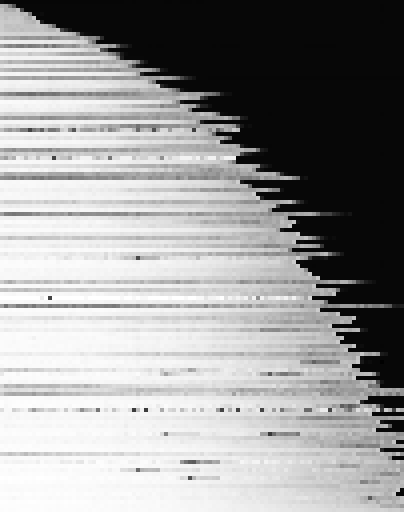
\includegraphics[width=3.35in]{profiles_128.png}}
\caption{Quality profiles obtained by $k$-means clustering on the
  fragment library from \textit{Rhodobacter sphaeroides} 2.4.1 data
  set using $k$ = 128, with each row corresponding to a quality
  profile. Dark to light colors represent low to high quality
  values. It is readily visible that the two most distinctive features
  of quality profiles is their drop-off position and average overall
  quality. One can also see sporadic low-position values in a handful
  of profiles, likely capturing intermittent problems in the
  sequencing process affecting thousands of reads at a
  time.}\label{fig:profiles_128}
\end{figure}

\subsection{Data sets}

We used several Illumina sequence read data sets in this research as
follows.

\textit{Rhodobacter sphaeroides} 2.4.1 data from the \textsc{gage}
(Genome Assembly Gold-Standard Evaluations)~\cite{Salzberg:2012rc},
which are generated from a fragment library (insert size of 180 nt;
2,050,868 paired-end reads) and short-jump library (insert size of
3,000 nt; 2,050,868 reads). The corresponding reference sequence was
obtained from the NCBI RefSeq database (NC\_007488.1, NC\_007489.1,
NC\_007490.1, NC\_007493.1, NC\_007494.1, NC\_009007.1, NC\_009008.1).

\textit{Homo sapiens} \ldots

\textit{Genus speices} \ldots

\subsection{Performance evaluation}

As a measure of compression effectiveness we use bits/base-call, and
define it as the size of the compressed representation of quality
values (in bits) divided by the number of quality values represented.
As a measure of information loss we use mean squared error
(\textsc{mse}) as aloss function, and define it as
$\frac{1}{n}\sum_{i=1}^{n}{(Q_i'-Q_i)^2}$, where $n$ is the number of
sequences, $Q_i'$ is the compressed/decompressed quality value, and
$Q_i$ is the original quality value associated with sequence position
$i$.

We evaluate effects of information loss from quality value compression
on quality control steps of read filtering and trimming, which were
performed using Sickle~\cite{sickle}, quantify read characteristics
with PrinSeq~\cite{Schmieder:2011gd}, and make comparison to
uncompressed data.

We evaluate effects of information loss from quality value compression
on \emph{de novo} genome assembly performance using contiguity
statistics, log average read probability
(\textsc{lap})~\cite{Ghodsi:2013hb}, and a collection of
reference-based metrics. The contiguity statistics include number of
scaffolds and NG50, which is defined as the weighted median contig
size (the length of largest contig $c$ such that the total size of the
contigs larger than $c$� exceeds half of the known genome size). The
\textsc{lap} score can be viewed as a log likelihood score, where a
value closer to 0 is better. We use a reference-based evaluation
script provided by \textsc{gage} that counts single nucleotide
polymorphisms (\textsc{snp}s), relocations, translations, and
inversions. The reference-based metrics are normalized by the length
of the assembly to aid in comparison. For the genome assembly we used
software that makes use quality values in the assembly process:
\textsc{allpaths-lg}~\cite{Gnerre:2011kx} version r50191 with default
settings and 32 threads.

\end{methods}

\section{Results}

\subsection{Compression effectiveness versus information loss}

We compare the \textsc{mse} versus bits/base-call of the fragment and
short-jump libraries of the \textit{Rhodobacter sphaeroides} 2.4.1
data set (Figures \ref{fig:mse_vs_bpbp_frag} and
\ref{fig:mse_vs_bpbp_jump}). Storing the uncompressed quality values
requires 1 byte per base-call because they are stored in
\textsc{ascii} format; however, lossless compression of the values
with BZip2 2.112 bits/base-call. 0-order polynomial regression and
32-profile encodings have the lowest bits/base-call. 5th-order
polynomial regression has the highest bits/base-call, but have among
the lowest \textsc{mse}. As the order of the polynomial increases, the
bits/base-call increase and the \textsc{mse} decreases at an
exponential rate.

\begin{figure}[!tpb]%figure2
\centerline{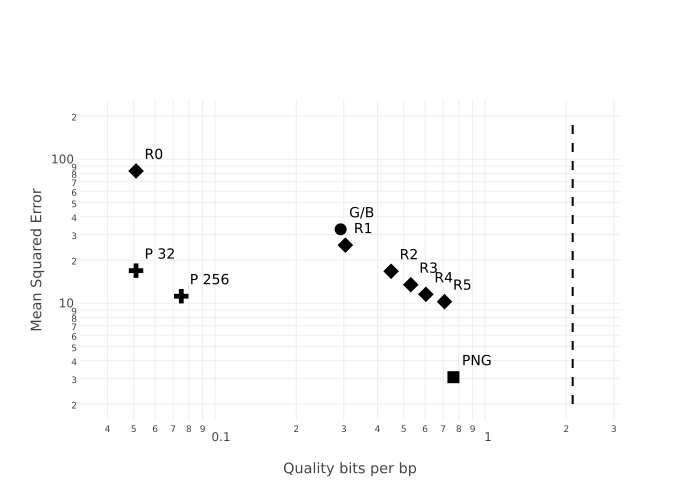
\includegraphics[width=3.65in]{mse_frag.png}}
\caption{Mean squared error versus bits/base-call for different
  compression methods applied to the fragment library from
  \textit{Rhodobacter sphaeroides} 2.4.1 data set. G/B: 2-bin
  encoding. P32 and P256: Quality profile compression with 32 and 256
  profiles. R0-R5: Polynomial regression-based compression using 0-5
  degrees. Dashed line corresponds to lossless bzip compression of
  quality values. \em}\label{fig:mse_vs_bpbp_frag}
\end{figure}

\begin{figure}[!tpb]%figure2
\centerline{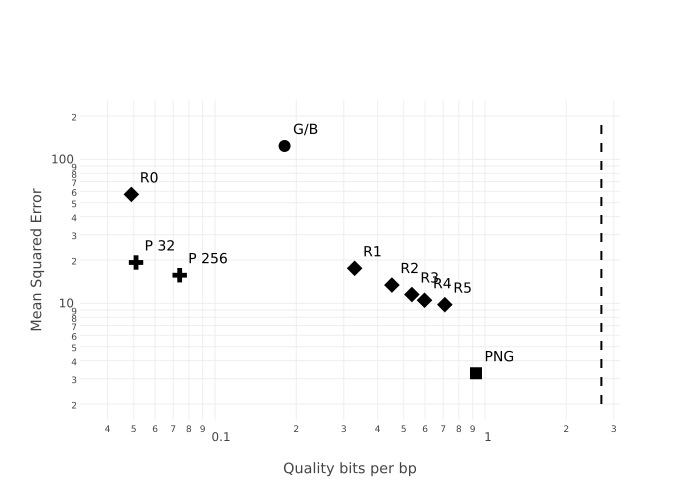
\includegraphics[width=3.65in]{mse_short.png}}
\caption{Mean squared error versus bits/base-call for for different
  compression methods applied to the short-jump library from
  \textit{Rhodobacter sphaeroides} 2.4.1 data set. G/B: 2-bin
  encoding. P32 and P256: Quality profile compression with 32 and 256
  profiles. R0-R5: Polynomial regression-based compression using 0-5
  degrees. Dashed line corresponds to lossless bzip compression of
  quality values. \em}\label{fig:mse_vs_bpbp_jump}
\end{figure}

\subsection{Effects on sequence read preprocessing}

Table \ref{tab:quality_control} shows the proportional numbers with
respect to those of the uncompressed \textsc{fastq} files. In the
fragment sample, we retain on average 95.4\% and 94.24\% of bases and
reads, respectively. In the short-jump sample, we retain 90.4\% and
90.98\% of bases and reads, respectively. In some cases, the
proportion of reads and/or bases compared to the original is more than
100\%; this means that the number of the reads and bases in the
compressed samples are more because altering quality values may
prevent the read from being filtered and/or trimmed. This is clear in
the good/ bad compression approach of the short-jump sample, where the
proportion of bases and reads are 113.09\% and 103.70\% respectively.

\subsection{Effects on genome assembly}

The assembly of the \textit{Rhodobacter sphaeroides} 2.4.1 data set
using the uncompressed reads outperforms all compression methods in
terms of \textsc{lap}, NG50, relocations, translations, and inversions
(Table \ref{tab:assembly_ranks}). Among the compression methods, the
256- and 32-profile encoding had the highest rank, then the 4th-order
polynomial regression, the 5th-order polynomial regression, the 2-bin
encoding, and lastly, the 3rd through 0-order polynomials.

The lossy compression methods largely preserve the contiguity found in
the assembly produced using the reads with unmodified quality
sequences. All compression methods other than 0-order polynomial
regression produce an NG50 ranging from 3.18--3.19 Mbps. Despite the
similar contiguity statistics, the different compression methods vary
noticeably in the amount of \textsc{snp}s. The order of polynomial has
an inverse relationship with the amount of \textsc{snp}s detected. The
2-bin and profile methods detected the least amount of \textsc{snp}s
compared to the reference genome, outperforming the assembly using the
original quality sequences. A more in-depth evaluation is needed to
determine whether these compression methods are missing actual
\textsc{snp}s.

It is important to highlight the result that the 4th-order polynomial
regression outperforms the 5th-order in all of the reference-based
metrics, but not the \emph{de novo} \textsc{lap} metrics. The
5th-order polynomial regression assembles approximately 2.5 kb more
sequence and uses roughly $1.2\%$ more of the total read set than the
4th-order (Supplemental Table 1), which may explain the discrepency in
\textsc{lap} values because the \textsc{lap} value is influenced by
total coverage~\cite{Ghodsi:2013hb}.

\begin{table*}[!tpb]
\centering
\caption[]{Rankings of different assemblies produced using proposed
  compression methods. Assemblies were constructed using
  \textsc{allpaths-lg} and the \textit{Rhodobacter sphaeroides}
  2.4.1. data set provided by
  \textsc{gage}~\cite{Salzberg:2012rc}. Regression methods are sorted
  by their overall rank (determined by the sum of individual
  rankings).}
{\begin{tabular}{lcccccccc}
& overall & & & & & & \textsc{lap} & \textsc{lap} \\
compression            & rank & \textsc{snp}s & inversions & relocations & translocations & indels & fragment & short-jump \\
\hline
none                   & 1    & 5    & 1          & 1           & 1              & 1      & 1          & 1                    \\
profile (256)          & 3    & 2    & 1          & 3           & 3              & 4      & 2          & 4                    \\
profile (32)           & 4    & 3    & 1          & 4           & 6              & 5      & 3          & 3                    \\
pegression (4th order) & 5    & 6    & 1          & 6           & 5              & 2      & 7          & 8                    \\
regression (5th order) & 6    & 7    & 1          & 5           & 7              & 7      & 5          & 7                    \\
2-bin	               & 7    & 1    & 1          & 8           & 11             & 10     & 6          & 5                    \\
regression (3rd order) & 8    & 8    & 1          & 9           & 9              & 6      & 8          & 6                    \\
regression (2nd order) & 9    & 9    & 1          & 7           & 4              & 8      & 9          & 10                   \\
regression (1st order) & 10   & 10   & 11         & 10          & 8              & 9      & 10         & 9                    \\
regression (0 order) & 11   & 11   & 10         & 11          & 10             & 11     & 11         & 11
\\ \hline
\end{tabular}
}
\label{tab:assembly_ranks}
\end{table*}

\subsection{Effects on read mapping}

Certain short read alignment tools use the quality sequence
information when finding potential alignments. Bowtie2 (version 2.2.3)
was used to evaluate the different decompressed \textsc{fastq}
files. Bowtie2 uses quality values written in the \textsc{fastq} files
when mapping reads against a reference genome. The original
uncompressed and decompressed \textsc{fastq} files were mapped with
Bowtie2 against \textit{Rhodobacter sphaeroides} reference genome. The
generated \textsc{sam} file for each compressing approach were
compared with the uncompressed \textsc{sam} file. The total, shared
and unique proportional numbers of mapped reads are calculated with
respect to the uncompressed \textsc{sam} matches as shown in table
\ref{tab:aligner}. Additionally, to monitor the effect of quality
values on mapping in general, Bowtie2 was tweaked with the maximum and
minimum mismatch penalty equivalent to maximum and minimum quality
scores (with parameters: --mp 6,6 and --mp 2,2 respectively).

Generally, increasing the regression model polynomial order from 0 to
5 results in more mapped reads with the most marked change from order
1 to order 2. The best compression approach is the one that has
highest proportion of reads shared between the uncompressed and
decompressed files and least number of reads that are unique in both
uncompressed and decompressed files. In fragment sample, on average,
99.03\% of reads were mapped using different compression approaches,
within which 99\% are shared with the uncompressed alignments and
0.02\% unique mapped reads in the decompressed file. The average
missed alignments are 0.99\%. Compression with profile 256 approach
was shown to be the best performing approach in the fragment
decompressed sample, as a proportional of 99.94\% reads are mapped
with respect to the uncompressed mapped reads within which 99.91\% are
common and only 0.08\% unique mapped reads in the decompressed
file. In short-run sample, the average number of mapped reads is 99.14
\% within which 98.73\% are common and 0.41\% unique mapped reads in
the decompressed file.The average missed alignments are
1.2\%. Regression with the 5th polynomial order captured the highest
mapped reads of 100\%, within which 99.66\% are common and only 0.33\%
unique mapped reads in the decompressed file.

\begin{table*}[!tbhp]
\centering
\caption[]{Mapping results of decompressed \textsc{fastq} files
  against \textit{Rhodobacter sphaeroides} reference genome using
  Bowtie2. Numbers corresponds to the proportion of mapped reads with
  respect to the uncompressed \textsc{fastq}. ``Shared'' denotes the
  percentage of mapped reads by both the uncompressed and decompressed
  data. ``Uncompressed only'' denotes the percentage of reads mapped
  from the uncompressed data that are not mapped after
  decompression. ``Compressed only'' denotes the percentage of reads
  mapped from the decompressed data that were not mapped before
  compression.}
\begin{tabular}{llcccc}
    & & \multicolumn{4}{c}{percentage of reads mapped}\\
    \cline{3-6}
	library & compression strategy & total & shared & uncompressed only & compressed only \\ \hline
	& maximum quality & 77.88 & 77.88 & 22.12 & 0 \\
	&minimum quality & 100 & 100 & 0 & 0 \\
	&2-bin & 99.92 & 99.89 & 0.11 & 0.03 \\
	&regression (0 order) & 93.63 & 93.62 & 6.38 & 0.02 \\
	&regression (1st order) & 98.62 & 98.61 & 1.39 & 0.01 \\
	&regression (2nd order) & 99.42 & 99.39 & 0.61 & 0.03 \\
	fragment&regression (3rd order) & 99.56 & 99.53 & 0.47 & 0.03 \\
	&regression (4th order) & 99.71 & 99.68 & 0.32 & 0.03 \\ 
	&regression (5th order) & 99.79 & 99.75 & 0.25 & 0.03 \\
	&profile (32) & 99.9 & 99.86 & 0.14 & 0.04 \\ 
	&profile (256) & 99.95 & 99.92 & 0.08 & 0.03 \\

\\ \hline \\

	&maximum quality & 78.08 & 78.08 & 21.92 & 0 \\
	&minimum quality & 100 & 100 & 0 & 0 \\ 
	&2-bin & 97.38 & 97.38 & 2.62 & 0 \\
	&regression (0 order) & 96.07 & 94.11 & 5.89 & 1.96 \\
	&regression (1st order) & 99.24 & 98.98 & 1.02 & 0.26 \\ 
	&regression (2nd order) & 99.66 & 99.35 & 0.65 & 0.3 \\ 
	short-jump&regression (3rd order) & 99.94 & 99.61 & 0.39 & 0.33 \\ 
	&regression (4th order) & 99.99 & 99.64 & 0.36 & 0.35 \\ 
	&regression (5th order) & 100 & 99.67 & 0.33 & 0.33 \\ 
	&profile (32) & 99.74 & 99.44 & 0.56 & 0.3 \\
	&profile (256) & 99.76 & 99.52 & 0.48 & 0.24 \\
\end{tabular}

\label{tab:aligner}
\end{table*}


\begin{table}[!tbhp]
\centering
\caption[]{Quality filtering/trimming for the uncompressed and
  decompressed \textsc{fastq} files. Numbers correspond to the
  proportion of bases/reads that are missed or gained after applying
  compression with respect to the uncompressed values.}
\label{tab:quality_control}
\begin{tabular}{lcccc}
	 & \multicolumn{2}{c}{fragments} & \multicolumn{2}{c}{short-Jump} \\
	 & \% bases & \% reads & \% bases & \% reads \\ \hline
	2-bin & 98.15 & 98.78 & 113.09 & 103.7 \\ 
	regression (0 order) & 86.71 & 62.64 & 43.31 & 27.51 \\
	regression (1st order) & 92.96 & 95.09 & 81.31 & 91.79 \\ 
	regression (2nd order) & 93.93 & 96.87 & 86.31 & 94.75 \\
	regression (3rd order) & 93.5 & 95.68 & 88.7 & 94.51 \\ 
	regression (4th order) & 94.43 & 96.7 & 91.94 & 97.02 \\ 
	regression (5th order) & 95.56 & 98.09 & 93.92 & 98.02 \\ 
	profile (32) & 99.12 & 98.96 & 102.89 & 102.24 \\
	profile (256) & 100 & 99.8 & 102.66 & 101.27 \\
\end{tabular}
\end{table}

\section{Discussion}

\subsection{Lossy compression acceptable for subsequent biological analyses}

The primary concern of using lossy compression methods is naturally
the extent of information loss, that we quantified by \textsc{mse} in
this study. \textsc{mse} and compressibility provide information in
the theoretical context to the methods, but they are not the end-all
of evaluation criteria. The performance of compressed datasets in
different subsequent analyses and applications are just as
important. Our benchmarks showed that some of the compression methods
with high error rates are still practical for certain kinds of
applications. Many subsequent tools proved to have enough additional
redundancy built-in to handle such loss in information. Passing the
decompressed quality sequences through quality control software shows
that most methods filter nearly as many bases as using original
quality sequences. Assemblers performing sequencing alignment use
percent similarity scores that are typically robust to standard
sequencing errors.

\subsection{Extension of 2-bin encoding}

2-bin encoding has the nice property of being simple to compute and
has good bits/base-call values. The 2-bin encoding suffers from having
a high \textsc{mse}, but fortunately, we have shown that in the case
of genome assembly, 2-bin encoding outperforms all polynomial
regressions encodings with degree less than 3. 2-bin encoding of the
fragment and short-jump libraries of \textit{Rhodobacter sphaeroides}
have \textsc{mse}s of $2.42\times$ and $10.76\times$ the 3rd-order
polynomial regression encodings, respectively. This further highlights
the importance of using additional contextual information of the
subsequent analyses when evaluating compressed quality values.

A potential extension to 2-bin encoding is to incorporate an
additional bin (\emph{okay}). The \emph{okay} value can be used where
the base qualities fall within a 2-bin range. Because the distribution
of quality values is skewed towards higher quality, we need to
experiment with different cutoffs for the \emph{okay} value and
determine if the additional storage is noticeable in subsequent
analyses.

\subsection{Potential for operations on compressed data}

Perhaps one of the greatest potential benefits of compressing quality
values is the potential to perform quality control and possibly other
operations directly on the compressed representations of the
data. This is easiest to to consider for profile-based
compression. The $k$ profiles can be evaluated for (pre-)processing
operations such as filtering and trimming, and the operations
transitively applied to the entire set of reads, thus saving
substantial computation associated with evaluating the full set of
reads.

\subsection{Future of lossy compression in bioinformatics analyses}

We have simply provided here the initial steps in analyzing the effect
of lossy compression on quality sequences using a single,
high-coverage bacterial data set. More work needs to be done using
additional biological data sets, such as human and mouse, along with
different sequencing technologies. A more direct comparison against
related lossy compression tools, such as
\textsc{SlimGene}~\cite{Kozanitis:2011kl} and
\textsc{QualComp}~\cite{Ochoa:2013rt}, needs to be
performed. Additionally, other types of sequencing data can be
analyzed apart from the Illumina data examined here. For example, the
PacBio sequencing instruments produce very long reads (with average
read lengths on the order of 10 kbp), but with the trade-off of having
a high error-rate ($\sim$15\%). Unlike the class of quality values we
have examined here, the distribution of erroneous bases is relatively
uniform~\cite{Ferrarini:2013vf}. Koren et al.~\cite{Koren:2013ye} have
shown that the assembly complexity of bacterial genomes can be greatly
simplified, producing near complete genome assemblies, by utilizing a
single run of these long reads. If long read sequencing technologies
such as PacBio become more widely adopted, it would be of huge benefit
to examine the potential of lossy compression algorithms on not only
the quality values, but the biological sequencing data themselves.


%%%%%%%%%%%%%%%%%%%%%%%%%%%%%%%%%%%%%%%%%%%%%%%%%%%%%%%%%%%%%%%%%%%%%%%%%%%%%%%%%%%%%
%
%     please remove the " % " symbol from \centerline{\includegraphics{fig01.eps}}
%     as it may ignore the figures.
%
%%%%%%%%%%%%%%%%%%%%%%%%%%%%%%%%%%%%%%%%%%%%%%%%%%%%%%%%%%%%%%%%%%%%%%%%%%%%%%%%%%%%%%

\section{Conclusion}

In this paper we have examined lossy compression on sequence quality
values and their effect on subsequent analyses. Although most previous
examinations on lossy compression primarily focused on information
loss, we have shown that typically used bioinformatics software today
have additional built-in sensitivity to handle significant loss of
information in the compressed quality values.

\section*{Acknowledgement}
We thank the organizers and participants of the 2014 University of
T\"{u}bingen and University of Maryland Bioinformatics Exchange for
Students and Teachers (BEST) Summer School.

\section{Some Alternative Text}

The following text is taken from a draft grant proposal, and the
content overlaps considerably with the other text in this
document. However, at least in some cases the wording of this
alternative text might be preferable and serve as a replacement. In
any event the entire draft manuscript has to be substantially revised.

\subsubsection{Pilot Study: profile-based compression of quality 
values}\label{sec:profile-based}

Quality value patterns can be readily determined by clustering
sequences of quality values and using the resulting cluster centers as
representative profiles. In our pilot study we used $k$-means
clustering, a vector quantization method that partitions a set of
samples into $k$ sets that minimize within-cluster sum of
squares~\cite{hastie_09_elements-of.statistical-learning}, as follows.

\begin{enumerate}
\item
Randomly sample an arbitrary number of quality sequences as a training
set.
\item
Perform $k$-means clustering on the sample, and use the cluster
centers as profiles for the dataset.
\item
Replace each quality value sequence with the index value of the
profile closest in Euclidean distance.
\end{enumerate}

Our pilot study results demonstrate that $k$ values as small as
32--256 sufficiently represent patterns in Illumina read quality
values such that performance in subsequent analyses is very close to
uncompressed data (see Section \ref{sec:pilot-evaluation}). The
resulting compressed quality component of the original set of
\textsc{fastq} files consists of the $k$ quality profiles (the fixed
size cost), and a single byte representing the assigned quality
profile index for each read (the marginal size cost). Therefore the
compression factor is proportional of read length: the marginal size
cost of 1 byte/read for Illumina HiSeq read lengths of 100 bp requires
0.01 bits/base-call, and MiSeq read lengths of 300 bp require 0.0033
bits/base-call. The fixed cost of profiles of course reduces the
compression ratio, but this fixed cost is amortized across reads in a
set. Both fixed and marginal costs can be further reduced with
subsequent compression of the index and profiles (e.g., using general
compression algorithms). Our pilot study demonstrates that using 256
profiles with subsequent bzip2 compression (using a Burrows-Wheeler
block-sorting compression algorithm, and Huffman coding) represents
quality values of Illumina 100 bp reads at 0.074 bits/base-call
compared to the original data compressed with bzip2 only of 2.11
bits/base-call for the fragment library and 2.70 bits/base-call for
the short jump library. The very recently published
Read-Quality-Sparsifier
(\textsc{rqs};~\cite{DBLP:conf/recomb/YuYB14}), which apparently
represents the current state-of-the-art for compressing quality
values, achieved best case compression of 0.254 bits/base-call, and a
mean compression of 1.841 bits/base-call. Whereas our profile method
achieves $\sim$3.432$\times$ more compression than textsc{rqs} best
performance, and $\sim$24.878$\times$ more than average
performance. Note too that the compression ratio for \textsc{rqs}
varies with the $k$-mer composition of the data, whereas profile-based
compression is invariant to $k$-mer composition.

\subsubsection{Evaluating compression effects on subsequent 
analysis results}\label{sec:pilot-evaluation}

Lossy compression compromises representation accuracy for better space
efficiency. Different lossy compression methods have different
properties, therefore we need to evaluate performance in a number of
analysis contexts, and use multiple performance measures to
appropriately evaluate lossy compression methods. Important
bioinformatics contexts include typical tasks, such as quality control
processing, \textit{de novo} genome assembly, and aligning reads to a
reference. In our pilot study we again used Illumina reads from
fragment and short-jump libraries of the \textit{Rhodobacter
  sphaeroides} as test data, and assessed the effects of lossy
compression on each of the aforementioned bioinformatics
operations. The results for the profile-based compression follow.

\paragraph{Aligning reads to a reference sequence}
Another important analysis involving read data are the alignments of
reads to a reference sequence. Such alignments are performed for
genome annotation, quantification of gene expression in RNA-Seq
studies, estimation of sequencing coverage, and other purposes. To
evaluate the effect of compression on read alignment we used
\textsc{bowtie} 2~\cite{Langmead:2012rw} with default settings and
max- and min-mismatch parameters of \texttt{-mp 6,6} and \texttt{-mp
  2,2} respectively. The proportion of reads mapped using
compressed/decompressed data was extremely close to that of the
uncompressed data: 0.999 for the fragment library reads, and 0.998 for
the short-jump library reads.

%\bibliographystyle{natbib}
%\bibliographystyle{achemnat}
%\bibliographystyle{plainnat}
%\bibliographystyle{abbrv}
%\bibliographystyle{bioinformatics}
%
\bibliographystyle{plain}
%
\bibliography{compression}


\end{document}
